\chapter{Results of the \ac{daq} tests}


\section{GANDALF Clock Frequency and ADC Test}
Before using the \ac{gandalf} modules in the \ac{daq}, they need to be tested.
For this to things are relevant.
One of these is the sample frequency, if it correspondes to the theoretical sample frequency.
The other is the test of the \acp{adc} to see if they have dead bits or other malfunctions.
To perform this test a \SI{150}{\mega\hertz} sin voltage signal was generated with an AWG and a \SI{150}{\mega\hertz} filter by XXXXXXX was used.
This filter ensures that the sin signal is clean and no unwanted frequencies are present.
The clean sin signal was than connected to the inputs of the \acp{gandalf}, one after another.
For each input \num{1000}1000 measurements were done each with XXXXX samples.
For each channel a \ac{fft} was done for one waveform using the python3 functions \textit{scipy.fft.rfft} and \textit{scipy.fft.rfftfreq} to find the frequencies in the signal.
\autoref{fig:gandalf_input_g23_ch0} shows the plot with the \ac{fft} for channel 0 of the \ac{amc} 46 used with the \ac{gandalf} 24.
In the plot the red line marks the \SI{150}{\mega\hertz} of the sin signal and the green line marks the peak frequency of the measured signal.
The measured values and the corresponding uncertainties are listed in \autoref{tab:gandalf_sin_150}.




To test if the bits in the \acp{adc} are working, the amplitudes of all samples of every waveforms in a measurement were put into histogram.





\section{Input Offset Voltage}
The first measurement with the \ac{emusic} board is to find out the input offset voltage of the \ac{emusic} for different \ac{dac} values.
This needs to be done to find out the exact overvoltage of the \acp{sipm}.
In order to perform this measurement, the setup in \autoref{fig:input_offset_setup} was assembled.
The \ac{emusic} board was powered by the \SI{8}{\volt} power supply and the XXXXXXXX power supply was used to supply the high voltage.
It was set to \SI{16}{\volt} since it was unimportant for the high voltage to be over the breakdown voltage of the \acp{sipm}.
It should only be over the maximum input offset the \ac{emusic} can generate for the resulting voltage to be applied in reverse direction to the \acp{sipm}.
For this measurement the \ac{emusic}s input \ac{dac} settings, which can range from 0 to 511, were set to 0.
Then the voltages between the negative high voltage pole and the voltage on the cathode of the \acp{sipm} were measured.
This measurement was done for one \ac{sipm} of each \ac{sipm} group.
The chosen \ac{sipm} were 1, 6, 11, 16, 21, 26, 31 and 36.
After measureing the voltages, the \ac{dac} setting was increased in steps of \SI{50}{\dacu} until \SI{500}{\dacu}.
For each setting the eight voltages were measured again.

The measurement for 




\section{Pole-Zero Cancellation}

In this section pole-zero cancellation shaper and its effect with different settings tested.
The tests were done using the setup described in \autoref{sec:setup}.
For the amplification the \ac{emusic} board 2 was chosen and the digitization was done by a GANDALF module.
The \ac{emusic} settings of one of these measurements are shown in \autoref{} in the appendix.
For the other measurements, the only thing changing in the settings are the pole-zero settings.
Each measurement includes XXXXX events, for which the mean value is shown in the plots below.
The values for the amplitude and \ac{fwhm} were calculated for each individual waveform and theire mean values are presented here for the different measurements.

First the pole-zero cancellation was disabled to perform measurements for a reference amplitude and \ac{fwhm}.
In \autoref{fig:pz_no_pz} the mean of all waveforms, measured in channel 0, is shown.
The mean amplitude is 
\begin{align}
    V_{amp} &= \SI{1(1)}{\milli\volt}
\end{align}
and the \ac{fwhm} is
\begin{align}
    t_\text{FWHM} &= \SI{1(1)}{\nano\second}.
\end{align}

Next the measurement with enabled pole-zero cancellation and with fixed settings for its capacitor and variing resistor values.
The resistor settings were changed to all possible values, from 0 to 7, and the capacitor setting was kept at 31.
\autoref{fig:pz_resistor} presents the mean waveforms for the eight measurements.
The determined amplitudes and \ac{fwhm} and the coresponding decrease in respect to the values without pole-zero cancellation are listed in \autoref{tab:pz_resistor}.
Of all measurements the one with the resistor setting 0 had the highest mean amplitude with 
\begin{align}
    V_\text{amp,R=0} &= \SI{1(1)}{\milli\volt}
\end{align}
which correspondes to a amplitude attenuation of \SI{1(1)}{\percent}.
With these settings a \ac{fwhm} of
\begin{align}
    t_\text{FWHM,R=0} &= \SI{1(1)}{\nano\second}
\end{align}
was measured, which is \SI{1(1)}{\percent} of the \ac{fwhm} measured without pole-zero cancellation.
\begin{figure}
	\centering
	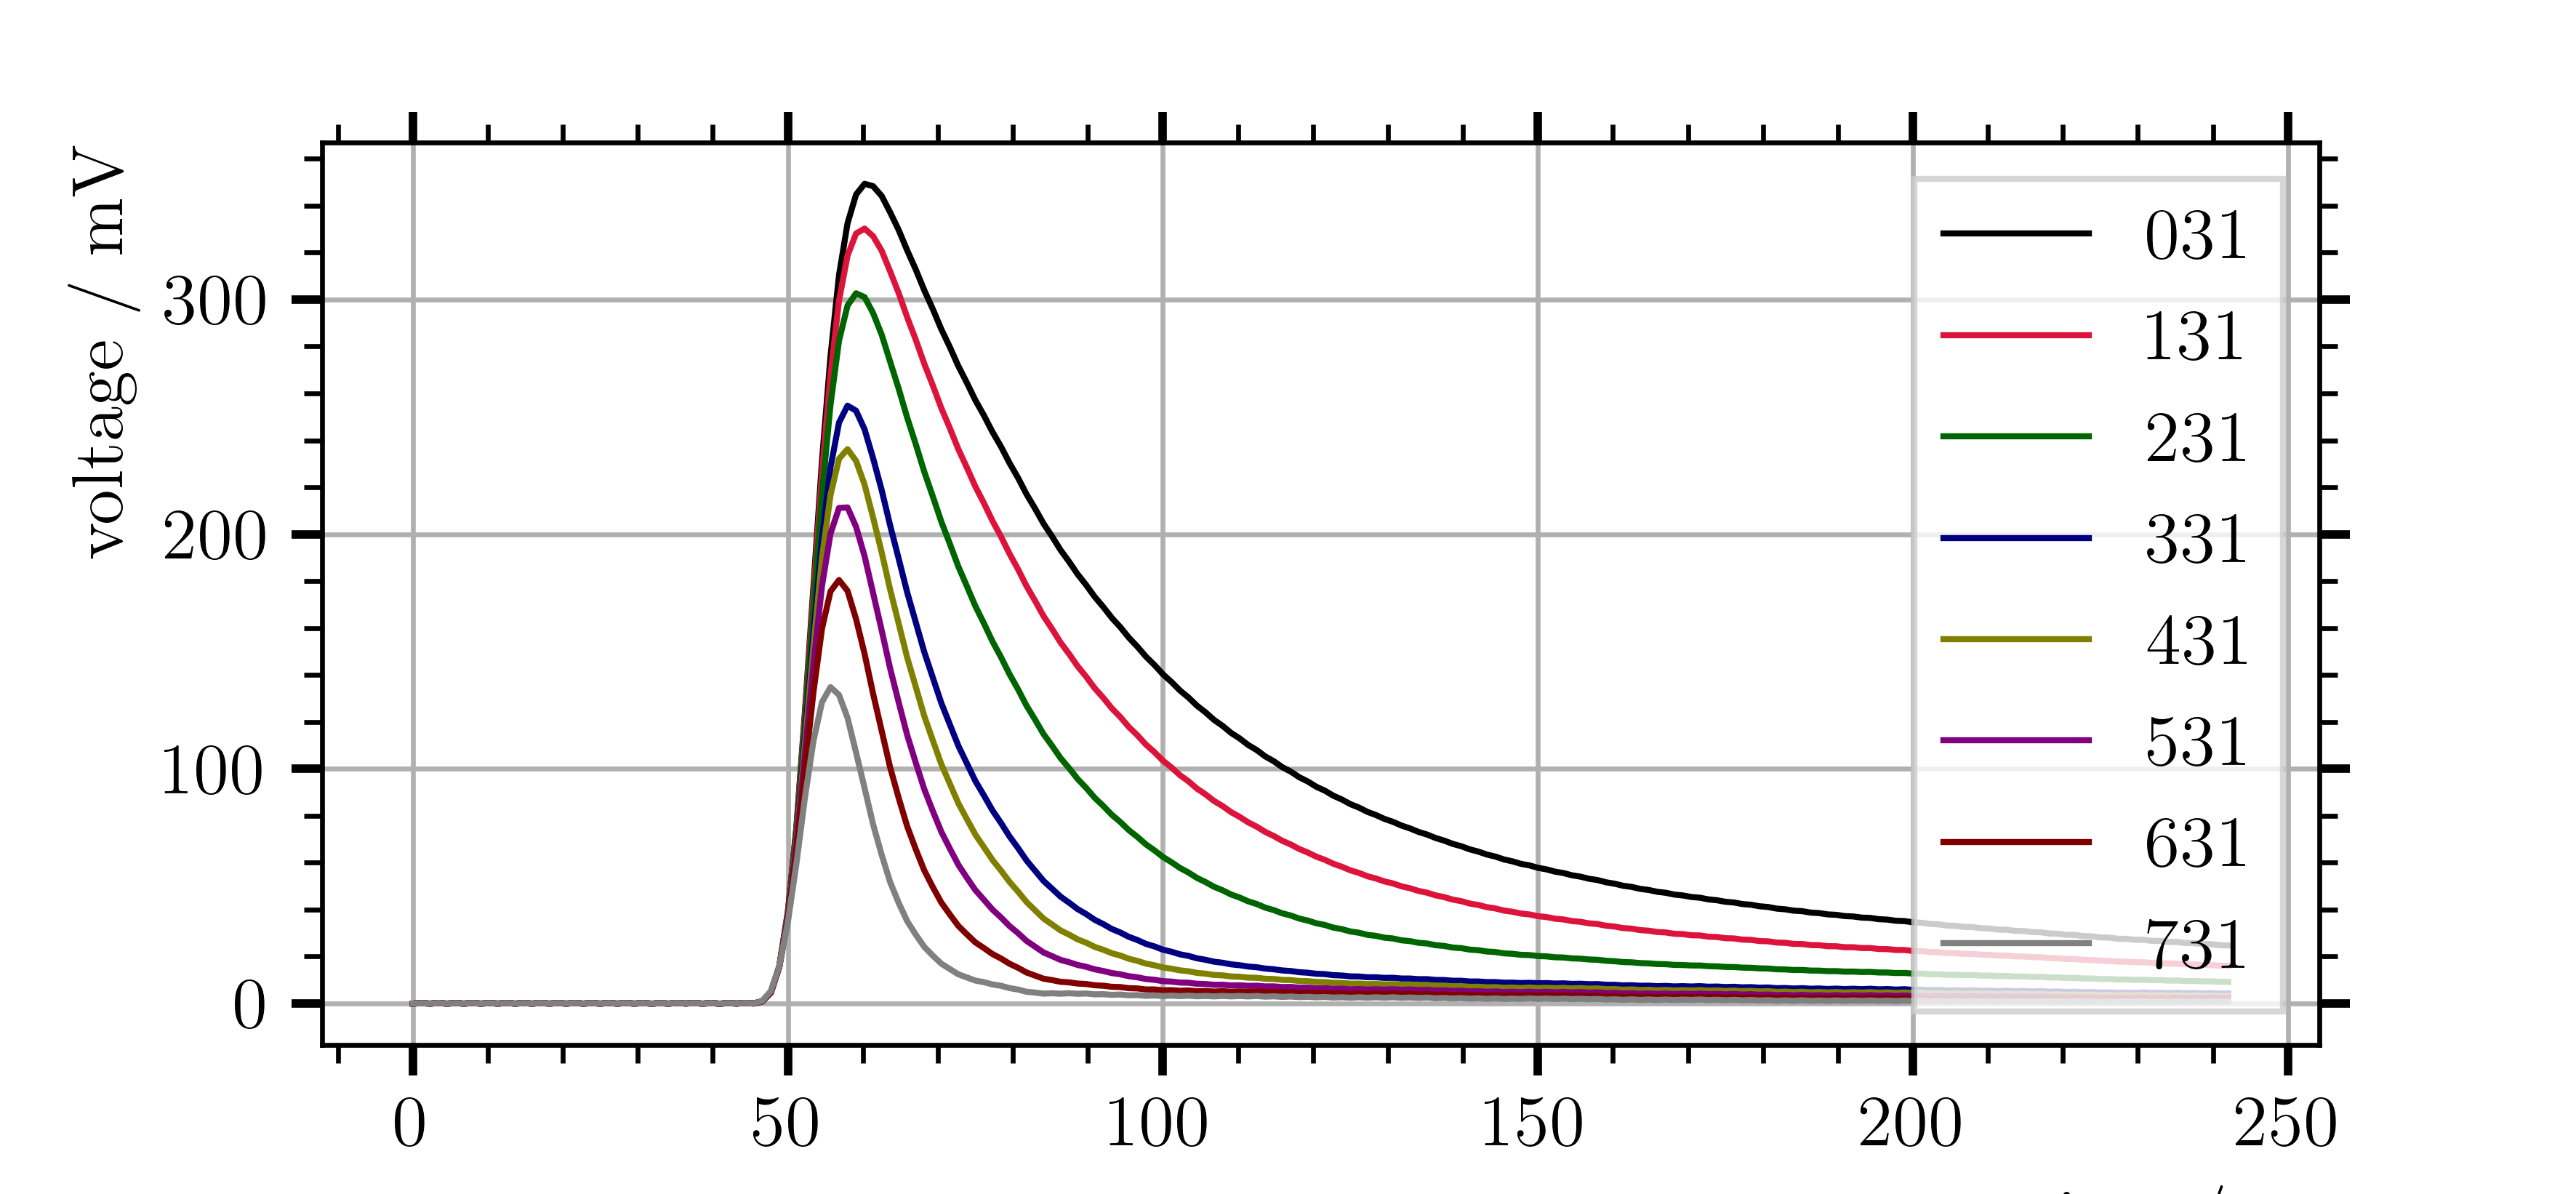
\includegraphics[width=1.\textwidth]{pictures/pz_resistor.png}
	\caption[Mean waveform for different pz-cancellation resistor values.]{Mean waveform for different pz-cancellation resistor values.}
	\label{fig:pz_resistor}
\end{figure}

The measurements with different capacitor settings were performed with the resistor setting of 0.
For the different measurements, the capacitor settings were changed to all 32 possible values, from 0 to 31.
In \autoref{tab:pz_capacitor} the mean values for the maximum amplitude and the \ac{fwhm} as well as the decrease compared to the values with disabled pole-zero cancellation are listed.
The mean waveforms for the measurements with the capacitor settings 0, 5, 10, 15, 20, 25, and 31 are shown in \autoref{fig:pz_capacitor}.
\begin{figure}
	\centering
	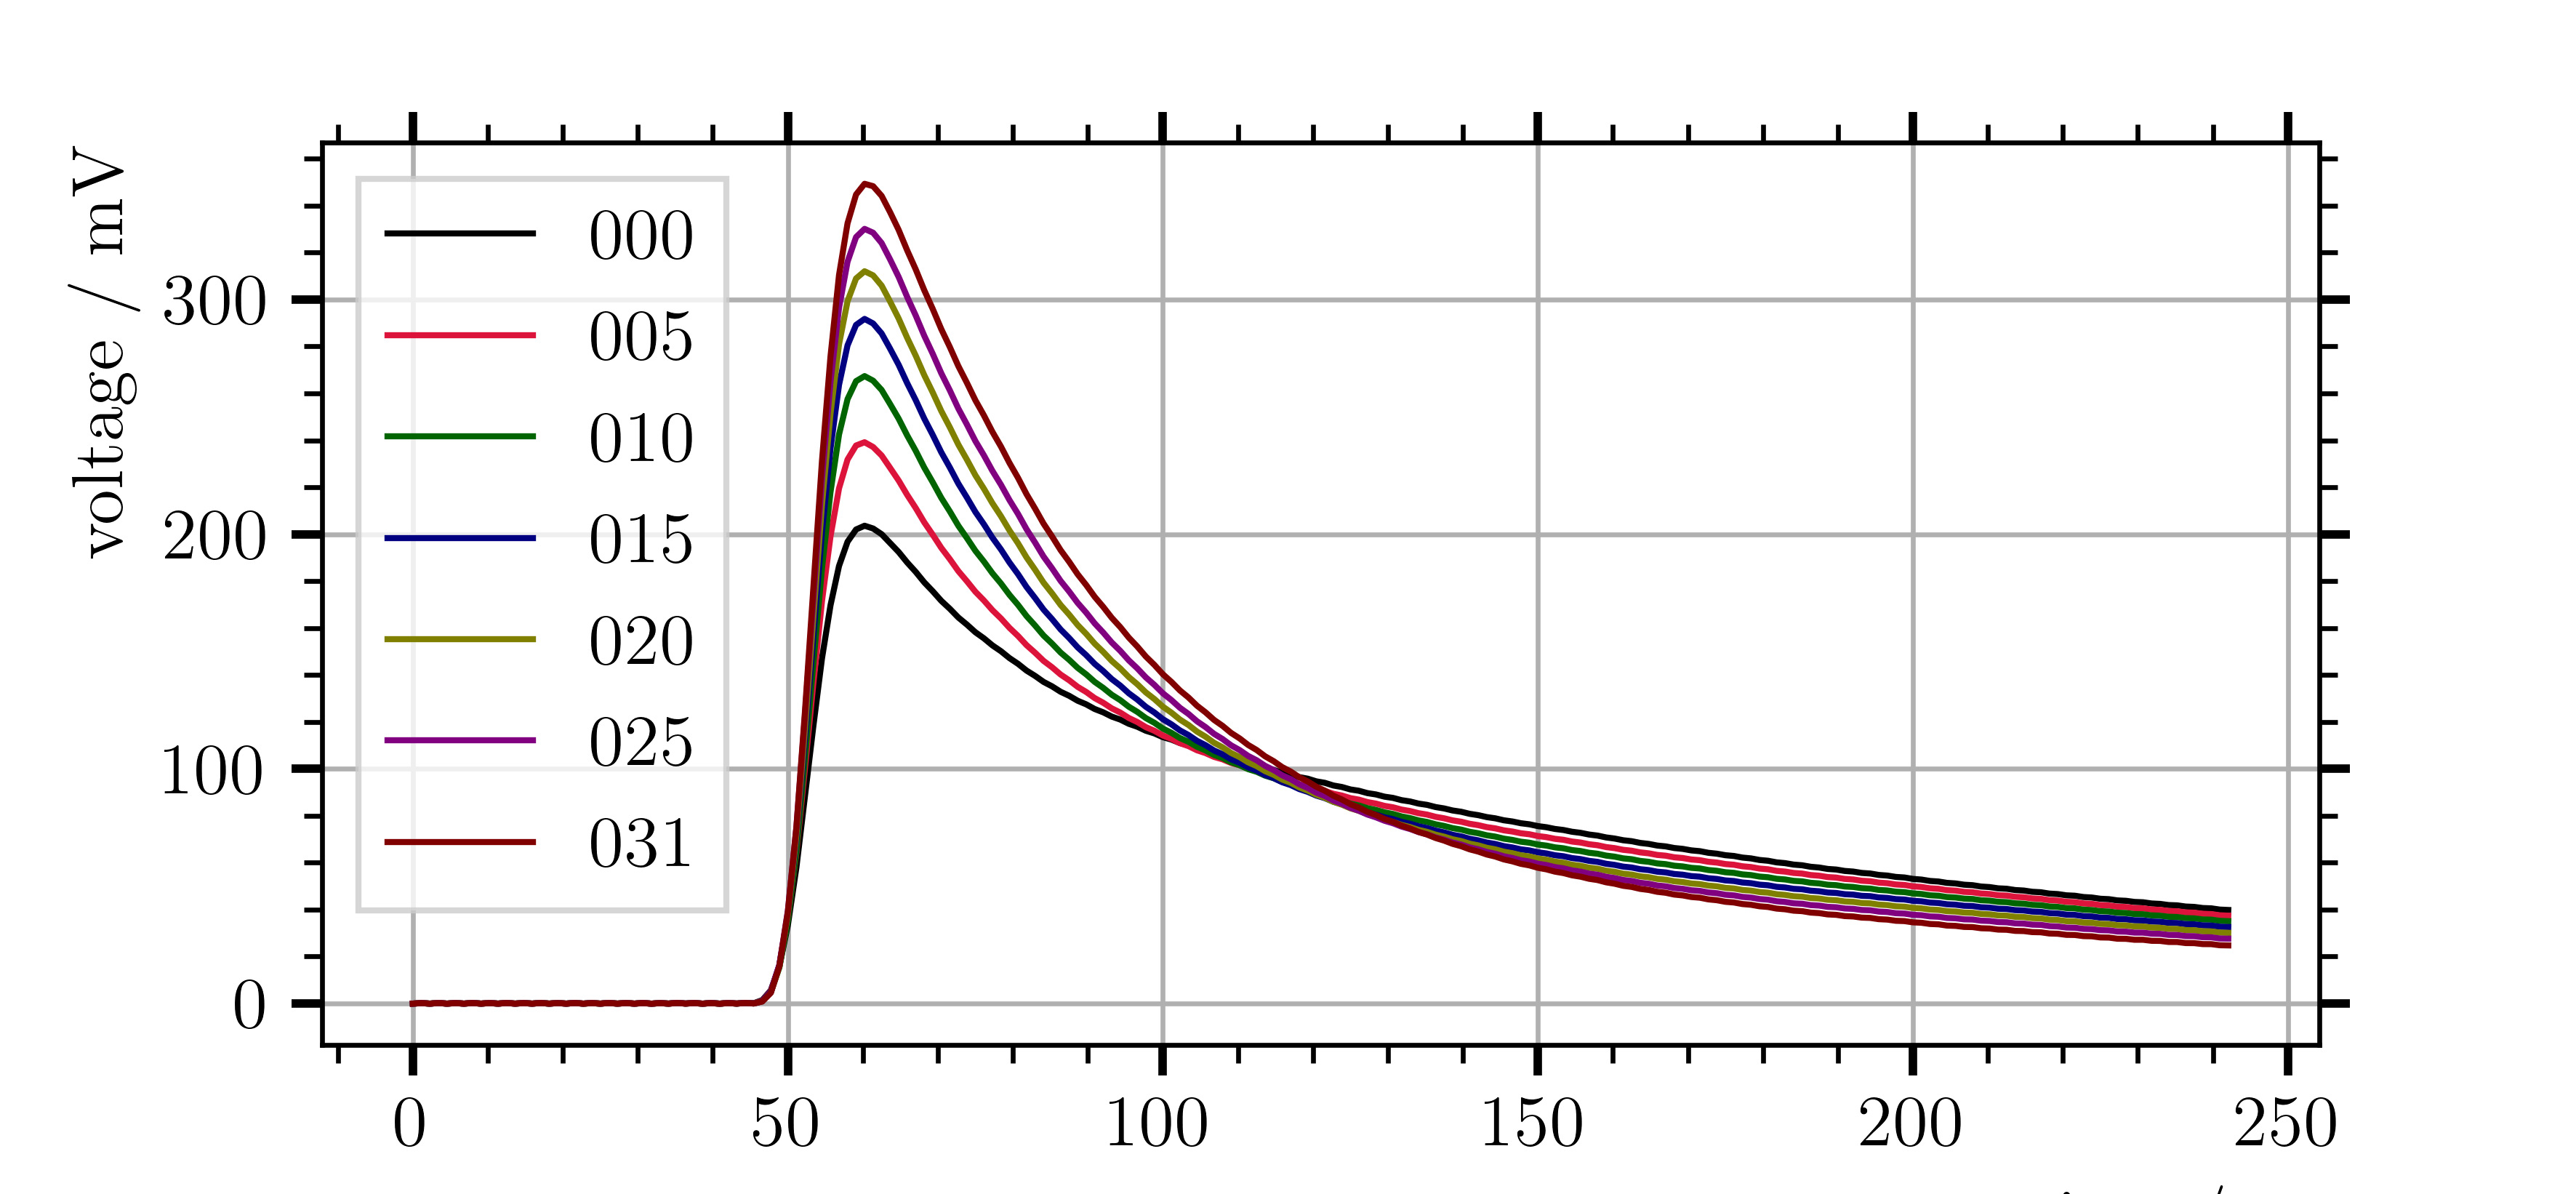
\includegraphics[width=1.\textwidth]{pictures/pz_capacitor.png}
	\caption[Mean waveform for different pz-cancellation capacitor values.]{Mean waveform for different pz-cancellation capacitor values.}
	\label{fig:pz_capacitor}
\end{figure}





\section{High and Low Transimpedance and Lower Attenuation}



\section{Dark Count Measurements}

